
\let\textcircled=\pgftextcircled
\chapter{System design}

\initial{A}s mentioned in Section \ref{sec:methodology}, the design of the Obstacle Collision Avoidance System will follow the Systems Engineering approach.
The main reason is that Systems Engineering provides some methods that prevent the errors with the highest consequences when the system to be designed is complex.
As explained by Rolls-Royce Global Chief of Systems Engineering \cite{beasley2015}:
\begin{quote}
	\itshape
	Systems Engineering collects and organises all the information needed to understand the whole problem, explores it from all angles, and then finds the most appropriate system solution.
\end{quote}

Furthermore, A key study published through INCOSE \cite{incoseuk2016} looked at the phase of detection of errors, and the consequent cost of fixing them.
Cost modelling was validated against a cross-industry range of defence and aerospace projects.
Figure \ref{fig:incose} shows the results of the study.

\begin{figure}[htbp]
	\centering
	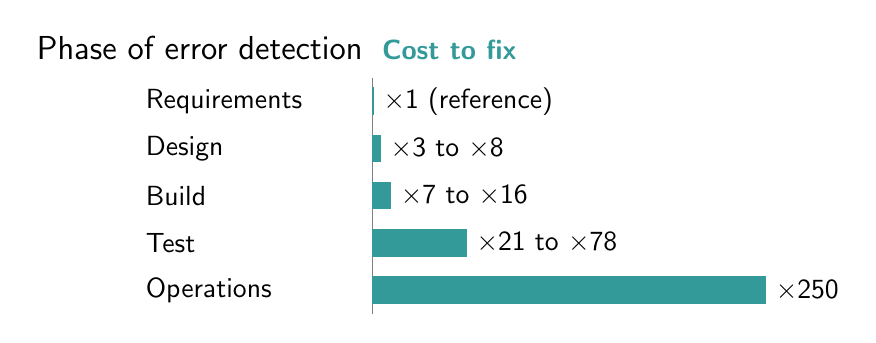
\begin{tikzpicture}

		\colorlet{blueish}{teal!80}

		%\draw[step=1cm,gray,very thin] (0,0) grid (9,6);

		\node[above left,black] at (3,6.2) {\sffamily \large Phase of error detection};
		\node[above right,blueish] at (3,6.2) {\sffamily \bfseries Cost to fix};
		\draw[black!50] (3,6.1) -- (3,3.1);
		\draw[blueish, line width=0.35cm] (3,5.8) -- (3.02,5.8);
			\node[right] at (0,5.8) {\sffamily Requirements};
			\node[right] at (3.02,5.8) {\sffamily $\times$1 (reference)};
		\draw[blueish, line width=0.35cm] (3,5.2) -- (3.11,5.2);
			\node[right] at (0,5.2) {\sffamily Design};
			\node[right] at (3.11,5.2) {\sffamily $\times$3 to $\times$8};
		\draw[blueish, line width=0.35cm] (3,4.6) -- (3.24,4.6);
			\node[right] at (0,4.6) {\sffamily Build};
			\node[right] at (3.24,4.6) {\sffamily $\times$7 to $\times$16};
		\draw[blueish, line width=0.35cm] (3,4) -- (4.2,4);
			\node[right] at (0,4) {\sffamily Test};
			\node[right] at (4.2,4) {\sffamily $\times$21 to $\times$78};
		\draw[blueish, line width=0.35cm] (3,3.4) -- (8,3.4);
			\node[right] at (0,3.4) {\sffamily Operations};
			\node[right] at (8,3.4) {\sffamily $\times$250};

	\end{tikzpicture}
	\caption{Cost to fix a design error. {\footnotesize Source: \cite{incoseuk2016}}}
	\label{fig:incose}
\end{figure}


Hence, in the present chapter, some of the most relevant Systems Engineering tools from the NASA Systems Engineering Handbook \cite{nationalaeronauticsandspaceadministration2007} will be applied


\section{Requirements capture}

The design process for a system is requirement driven, since the requirements are what will define the cost, design, schedule\ldots\ % Space after \ldots
A requirement is a statement about or a characteristic of something that is needed.

Requirements can be derived from a variety of sources, like customer needs, stakeholders, regulations, procedures, constrains, etc.
However, for this project, customers and stakeholders will be disregarded (since none exist) and the motivation as stated in Section \ref{sec:motivation} will be used instead.

In the present section some requirements will be posed, but only those that directly apply to the OCAS subsystem or its interfaces, since the platform is considered to be completely functional prior to the introduction of the solution (following the modularity concept).

%\begin{table}[htbp]
\begin{center}
\begin{longtable}{>{\centering}m{0.7cm}|m{8cm}|>{\centering}m{2.7cm}|>{\centering}m{2.5cm}@{ }c@{ }}

	\hline
	\cellcolor{teal!10}{Req. ID}	&	\centering Requirement	&	Traceability (sourced from)	&	Traceability (allocated to)	&\\ \endfirsthead \endhead

	\hline
	\multicolumn{5}{l}{\cellcolor{black!15}{\footnotesize Certification}} \\
	1.1	&	The UAV shall meet European regulations	&	EC No 218/2008	&	\\
	1.2	&	The UAV shall meet Spanish regulations	&	Ley 18/2014		&	\\

	\hline
	\multicolumn{5}{l}{\cellcolor{black!15}{\footnotesize Architecture}} \\
	2.1	&	The OCAS shall work independently of the UAV	&	Motivation	&	\\
	2.2	&	The OCAS shall be self-contained within the UAV	&	Integration	&	\\

	\hline
	\multicolumn{5}{l}{\cellcolor{black!15}{\footnotesize Functionality}} \\
	3.1	&	The OCAS shall detect obstacles surrounding the UAV	&	Motivation	&	\\
	3.2	&	The OCAS shall avoid collisions with the detected obstacles	&	Motivation	&	\\
	3.3	&	The OCAS shall not interfere with existing Ardupilot functions	&	Motivation	&	\\
	3.4	&	The UAV shall maintain a communications data-link with the GCS at all time	&	Safety / FFBD	&	\\

	\hline
	\multicolumn{5}{l}{\cellcolor{black!15}{\footnotesize Performance}} \\
	4.1	&	The OCAS shall detect obstacles closer than 4 m to the UAV	&	Technical constraint	&	\\
	4.2	&	The OCAS shall detect obstacles of at least 0.5 m across	&	Technical constraint	&	\\
	4.3	&	The OCAS shall be powered along the full mission	&	Safety / FFBD	&	\\

	\hline
	\multicolumn{5}{l}{\cellcolor{black!15}{\footnotesize Interfaces}} \\
	5.1	&	The OCAS shall know the state of the UAV	&	FFBD	&	\\
	5.2	&	The OCAS shall send commands to the UAV	&	FFBD	&	\\
	5.3	&	The OCAS shall be accessible from the GCS	&	Human factors	&	\\
	5.4	&	The OCAS shall be activated and deactivated by the pilot	&	Safety / Human factors	&	\\

	\hline
	\multicolumn{5}{l}{\cellcolor{black!15}{\footnotesize Safety}} \\
	6.1	&	The OCAS shall improve the operational safety of the UAV	&	Motivation	&	\\
	6.2	&	The operation of the OCAS shall not be disrupting to the workflow of the pilot	&	Motivation	&	\\

	\hline
	\multicolumn{5}{l}{\cellcolor{black!15}{\footnotesize Reliability}} \\
	7.1	&	The OCAS shall avoid any physical collision	&	Motivation	&	\\
	7.2	&	The OCAS shall be operative regardless of the state of the controller board	&	Safety	&\\

	\hline
	\multicolumn{5}{l}{\cellcolor{black!15}{\footnotesize Ergonomics and human factors}} \\
	%\multicolumn{5}{l}{} \\
	8.1	&	The OCAS shall be operable after a short training by any pilot	&	Motivation	&	\\
	8.2	&	The OCAS should be engaged and disengaged at discretion of the pilot	&	Safety / FFBD	&	\\ 

	\hline
	\multicolumn{5}{l}{\cellcolor{black!15}{\footnotesize Loads}} \\
	9.1	&	The OCAS shall stand the same loads as the UAV	&	Integration	&	~	&\\

	\hline
	\multicolumn{5}{l}{\cellcolor{black!15}{\footnotesize Weight}} \\
	10.1	&	The UAV + OCAS shall not weight more than the limit of the UAV segment	&	Regulations	&	~	&\\

	\hline
	\multicolumn{5}{l}{\cellcolor{black!15}{\footnotesize Environment}} \\
	11.1	&	The OCAS shall withstand the effect of open-air flight	&	Integration	&	~	&\\

	\hline

	\caption{\cellcolor{white}{System-level requirements}}
	\label{tab:sysReqs}

\end{longtable}

\end{center}
%\end{table}


Notice that Table \ref{tab:sysReqs} is not static, and should be updated during the design process, since some of the tools of Systems Engineering are designed to expose missing requirements.
Thus, some requirements have been written at later design stages, as the ``Traceability (sourced from)'' column shows.
Also, the fourth column is to be completed in the subsystem design stage, when the system requirements will be allocated to one or more specific subsystems or components.


\section{Functional Analysis}

The Functional Analysis is an intermediate step between the Requirements Capture and the Design phases.
Its purpose is to understand the manner in which the requirements affect the way that the system functions, for the requirements loop; and to identify a feasible solution that functions in a way that meets the requirements, for the design loop.




